\documentclass[graphics]{beamer}

\usepackage{graphicx}
\usepackage{verbatim}
\usepackage{wrapfig}
\useoutertheme{shadow}
%\usecolortheme{orchid}
\usecolortheme{seahorse}


% math commands
\newcommand{\be}{\begin{eqnarray}}
\newcommand{\ee}{\end{eqnarray}}
\newcommand{\beq}{\begin{equation}}
\newcommand{\eeq}{\end{equation}}
\def\simless{\mathbin{\lower 3pt\hbox
      {$\rlap{\raise 5pt\hbox{$\char'074$}}\mathchar"7218$}}}
\def\simgreat{\mathbin{\lower 3pt\hbox
      {$\rlap{\raise 5pt\hbox{$\char'076$}}\mathchar"7218$}}} %> or of order

% variables

\def\toonscale{0.45}
\def\mboxy#1{\mbox{\small #1}}


\begin{comment}
\AtBeginSection[]{
  \frame{
    \frametitle{Outline}
    \tableofcontents[currentsection]
  }
}
\end{comment}

\title{21cm absorbers
}
%\subtitle{interim update}
\author[U. Pen]{Ue-Li Pen
\\[8mm] 
}
\date{May 18, 2021}


\begin{document}

%\section*{Introduction}
\section{Absorbers}

\begin{comment}
  \subsection{Outline}

  \frame{
    \frametitle{Outline}
    \tableofcontents
  }
\end{comment}

\frame{\maketitle}



  \frame{
    \frametitle{21cm Absorbers}
    \begin{itemize}
        \item 21cm transition: $\Delta T=h\nu/k=68$mK
        \item $Delta T \ll 2.78$K:  $3n_1/n_0=\exp(\delta E/kT)\sim
          1+0.068/T$
          \item optical depth $\tau \propto 1/T$
        \item emission $\propto $T, $\tau$ is independent of T, absorption $\propto 1/T$
        \item colded atoms in LoS dominate
        \item typically dominated by cold atomic clouds
    \end{itemize}
  }


  \frame{
\vspace{-0.5in}
    \frametitle{History}
    \begin{itemize}
    \item first detected in 3C278 at GBO in 1950
        \item current best constraint on direct measurement of cosmic
          acceleration (Darling 2012)
\item $z= 0.692153275(85)$, is $ż = (1.6 \pm 4.7) × 10^{−8}$/yr,
  expected $\dot{z}=2\times 10^{-11}$/yr.
        \item concept: watch the doppler shift of objects change with
          time:
          \item acceleration: doppler shift increases with time
          \item deceleration: doppler shift decreases with time
          \item bypasses need of general relativity
            
    \end{itemize}
  }


  \frame{
\vspace{-0.5in}
    \frametitle{Strategy}
    \begin{itemize}
    \item implemented high frequency resolution CHIME all sky survey
      (James, Arash, CIRADA, etc): 3 kHz
        \item need exquisite system stability
        \item how can we know our bandpass to $10^{-5}\sim
          1/\sqrt{\delta \nu t}$?
        \item RFI?
        \item use earth-sun doppler modulation
        \item 
        \item 
    \end{itemize}
\hspace{-0.2in}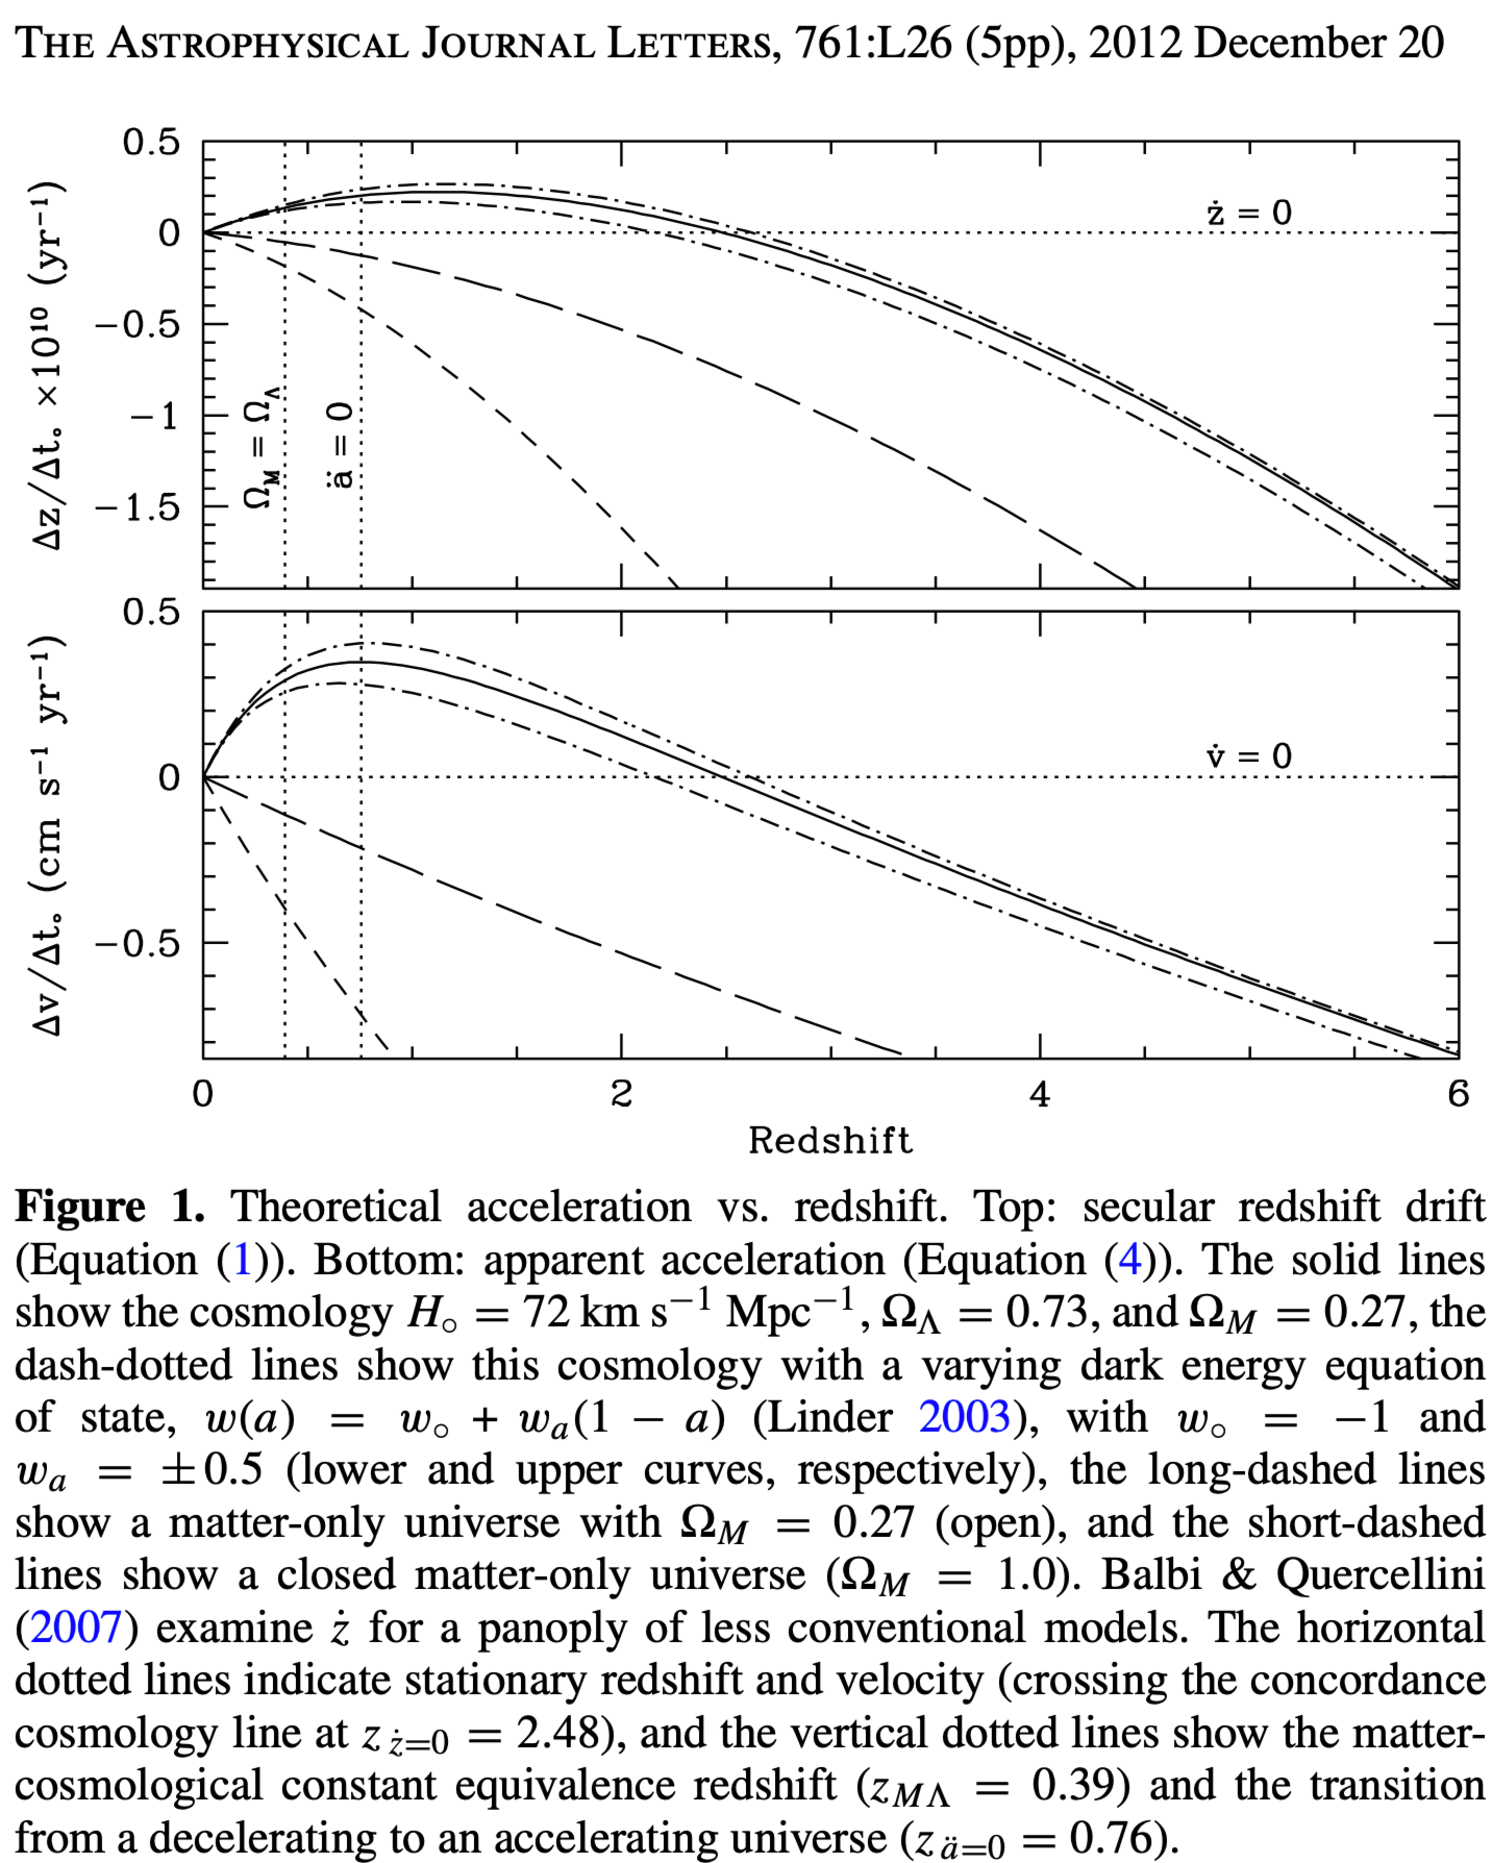
\includegraphics[width=4.5in]{Figures/darling.png}

  }


  \frame{
\vspace{-0.5in}
    \frametitle{Future potential}
    \begin{itemize}
    \item large number of 21cm absorbers
    \item measure gas temperature by comparison with L$_\alpha$
    \item test fine structure evolution
    \item nature of DLAs
    \item obscuration bias
    \item associated absorption: AGN accretion disk
    \item majority of radio loud QSOs have no optical redshift
    \item majority of DLAs cannot be imaged in the optical due to QSO
      blinding
    \item first large sample of unblinded DLA
    \item potentially discover OH maser emission/absorption: rest
      frame 1.612, 1.665, 1.667, 1.720 GHz lines
    \end{itemize}
  }

  \frame{
\vspace{-0.5in}
    \frametitle{Localization}
    \begin{itemize}
    \item CHIME resolution will limit absorber positions to several arcminutes
    \item potentially confusion limited identification of background source
    \item could localize with CHIME outriggers
    \item
    \end{itemize}
  }

  \frame{
\vspace{-0.5in}
    \frametitle{Conclusions}
    \begin{itemize}
    \item CHIME is by far world's fastest radio survey telescope
    \item absorbers are 
    \item 
    \item 
    \item 
    \item 
    \item 
    \item
    \item
    \end{itemize}
  }

\end{document}
